\section{Anwendung der Differential- und Integralrechnung}

\subsection{Beschreibungungsvarianten\formelbuch{49ff}}
  \begin{minipage}[t]{3.5cm}
    Funktion (explizit) \\
    $ y = f(x)$ \\
        \tiny{(Bronstein Form 2.4)}
  \end{minipage}
  \begin{minipage}[t]{6cm}    
    Koordinatengleichung (implizit) \\
    $ F(x,y) = 0 $ \\
        \tiny{(Bronstein Form 2.5)}
  \end{minipage}
  \begin{minipage}[t]{5.5cm}    
    Parameterform \\
    $ \left( \begin{array} {l} x(t) \\ y(t) \end{array} \right) =
          \left( \begin{array} {l} \Psi(t) \\ \varphi(t) \end{array} \right)$\\
        \tiny{(Bronstein Form 2.6)}
  \end{minipage} 
  \begin{minipage}[t]{3cm}
      Polarform x\\
      $ r=f(\varphi) $ \\
        %\tiny{(Bronstein Form 3.427)}
    \end{minipage}\\

  \textit{Hat man die explizite Form gegeben, so hat man automatisch die
  Implizite- und Parameter-Form}

\subsection{Umrechnen diverser Systeme \formelbuch{(197)}}
\begin{tabular}{lll}
x & $r \cos(\varphi)$ & \\
y & $r \sin(\varphi)$ & \\
r & $\sqrt{x^2 + y^2}$ & \\
Parameter 
  & $\Rightarrow$ explizit
  %& $x = f(t) \; \; y = g(t)$
  & $\Longrightarrow t = f(x);\; y = g(f(x))$\\
Ex- bzw. implizit 
  & $\Rightarrow$ Polar
  %& $y = f_1(x)$ bzw. $f_2(x,y) = C$
  & $\Longrightarrow$ Ersetze $x$ durch $r
\cos(\varphi)$ \& $y$ durch $r \sin(\varphi)$\\ 
Polar 
  & $\Rightarrow$ implizit
  %& $r = f(\varphi)$
  & $\Longrightarrow$ Ersetze $r \sin(\varphi)$ durch $y$, $r \cos(\varphi)$
  durch $x$, $r$ durch $\sqrt{x^2 + y^2}$\\ 
Polar
  & $\Rightarrow$ Parameterform
  %& $r = f(\varphi)$
  & $\Longrightarrow \left( \begin{array} {l} x(\varphi) \\ y(\varphi) \end{array} \right) =
          \left( \begin{array} {l} r(\varphi) \cos(\varphi) \\ r(\varphi) \sin(\varphi) \end{array}
          \right)$ \\
Explizit
  & $\Rightarrow$ Parameter
  %& $y = f(x)$
  & $\Longrightarrow \left( \begin{array} {l} x(t) \\ y(t) \end{array} \right) =
          \left( \begin{array} {l} x(t)) \\ t \end{array}
          \right)$ \\
Einzelner Punkt  
  & $\Rightarrow$ Polar
  %& $(x,\; y)$
  & $\Longrightarrow r = \sqrt{x^2 + y^2};\;
  \varphi = \begin{cases}\arctan(\frac{y}{x}) + \pi   &x < 0\\
             \arctan(\frac{y}{x})   & x > 0\\
             \frac{\pi}{2}      & x = 0;\; y > 0\\
             -\frac{\pi}{2}     & x = 0;\; y < 0\\
             \text{unbestimmt}    & x = y = 0\end{cases}$\\
\end{tabular}

\subsection{Kurvenarten\formelbuch{203ff}}
\begin{tabular}{llll}
\parbox{2.7cm}{
\textbf{ } \\
Implizit:\\
Bemerkung:\\
Polarform:\\
Parameterform:
}

\parbox{6cm}{
\textbf{Kreis\formelbuch{203}}\\
$(x-x_0)^2 + (y - y_0)^2 = r^2$\\
Mittelpunkt $(x_0, y_0)$; Radius $r$\\
$r = \frac{p}{1 + \epsilon \cos(\varphi)}; \epsilon = 0$ \\
$x=x_0 + R\cos(t), y=y_0 + R\sin(t)$
}

\parbox{8cm}{
\textbf{Ellipse\formelbuch{204}}\\
$(\frac{x-x_0}{a})^2 + (\frac{y-y_0}{b})^2 = 1$\\
Mittelpunkt $(x_0, y_0)$; Halbachsen $a$, $b$\\
$r = \frac{p}{1 + \epsilon \cos(\varphi)}; 0 < \epsilon < 1$\\
$x = a\cos(t), y = b\sin(t)$
}\\ \\

\parbox{2.7cm}{
\textbf {}\\
Implizit:\\
Bemerkung:\\
Polarform:\\
Parameterhform:
}

\parbox{6cm}{
\textbf{Hyperbel\formelbuch{206}}\\ 
$(\frac{x}{a})^2 - (\frac{y}{b})^2 = 1; -(\frac{x}{a})^2 + (\frac{y}{b})^2 =1$\\ 
\\
$r = \frac{p}{1 + \epsilon \cos(\varphi)}; \epsilon > 1$\\
$x= a \cosh(t), y = b \sinh(t) $
}

\parbox{8cm}{
\textbf{Parabel\formelbuch{209}}\\
$y= ax^2 + bx + c$\\
Parabeln mit Scheitelpunkt auf der vertikaler Achse\\
$r = \frac{p}{1 + \epsilon \cos(\varphi)}; \epsilon = 1$\\
$x=t, y = a t^2 + b t + c$
}\\ \\

\parbox{2.7cm}{
\textbf{} \\
Polarform:
}

\parbox{5cm}{
\textbf{Kardioide/Herzk. \formelbuch{99}} \\
$r = a(1+\cos(\varphi))$
}

\parbox{5cm}{
\textbf{Lemniskate ``$\infty$'' \formelbuch{101}} \\
$r = a\sqrt{2\cos(2\varphi)}$ 
}

\parbox{5cm}{
\textbf{Strophoide/harm. K. \formelbuch{96}} \\
$ r = -a \frac{\cos(2\varphi)}{\cos(\varphi)},(a>0) $ 
}

\end{tabular}

\subsection{Gleichungen\formelbuch{248}, Mittelwerte\formelbuch{19ff}}
\begin{tabular}{llll}
  \textbf{Tangentengleichung} &
  \textbf{Normalengleichung} &
  \textbf{Linearer Mittelwert} &
  \textbf{Quadratischer Mittelwert}\\
  $y-y_0=f'(x_0)(x-x_0)$ &
  $y-y_0=-\frac{1}{f'(x_0)}(x-x_0)$ &
  $\bar{f} = \frac{1}{b-a} \int\limits_{a}^{b} f(x)dx$ &
  $\bar{f} = \sqrt{\frac{1}{b-a} \int\limits_{a}^{b} f(x)^2dx}$
\end{tabular}
  
\subsection{Tangenten- \& Normalenabschnitt, Subtangente \&
Subnormale\formelbuch{249ff}}

\subsection{Abstandsformeln}
\begin{minipage}{6.5cm}
    \textbf{Hessesche Normalform\formelbuch{200f, 222}}\\
    $x\cdot \cos\varphi_0 +y\cdot \sin\varphi_0=r_0$\\
    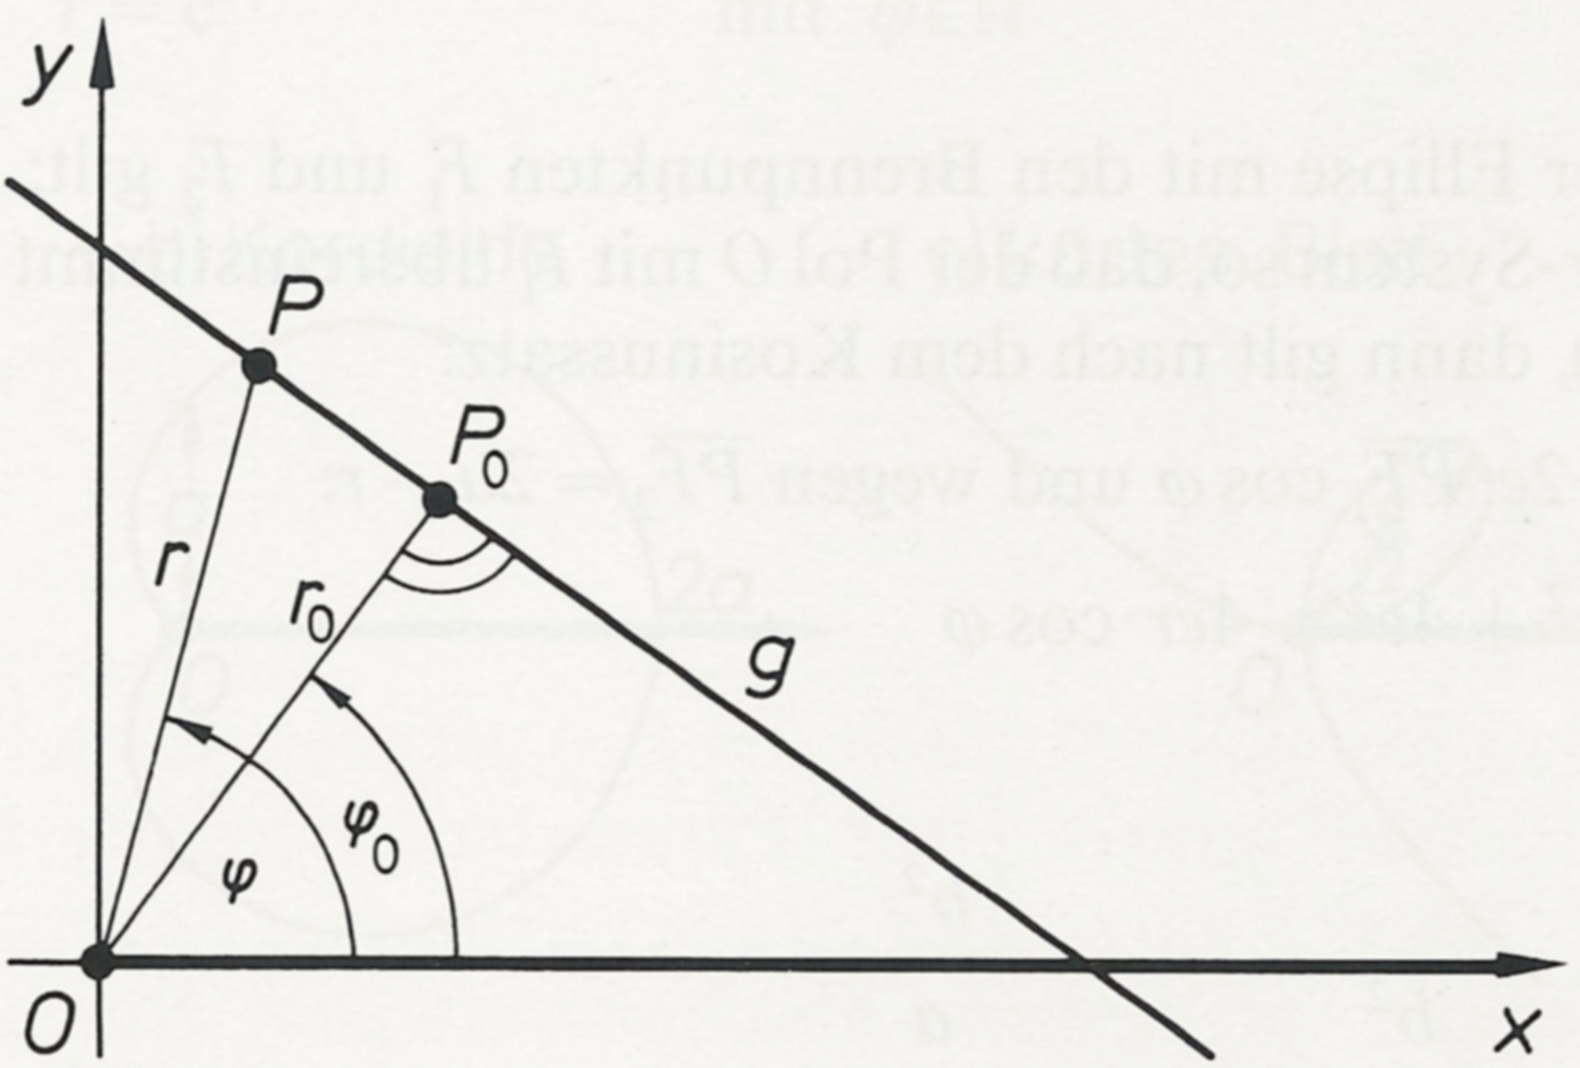
\includegraphics[width=2.8cm]{./bilder/hessenorm.png}
\end{minipage}
\begin{minipage}{6.5cm}
  \textbf{Geradengleichung} \\
  $y - y_0 = m (x - x_0)$
\end{minipage}
\begin{minipage}{6cm}
  \textbf{Abstand zum Ursprung} \\
  $\frac{|y_0 - m \cdot x_0|}{\sqrt{m^2 + 1}}$
\end{minipage}

\subsection{Ber"uhrung h"oherer Ordnung}
Zwei explizit gegebene Kurven $y = f(x)$ und $y = g(x)$ ber"uhren einander im
Punkt P $x_0, y_0$ von der Ordnung $n$, wenn die Funktionswerte und die ersten
$n$ Ableitungen existieren und �bereinstimmen.\\
$f(x_0) = g(x_0);\; f'(x_0) = g'(x_0);\; f''(x_0) = g''(x_0);\;\ldots ;
\;f^{(n)}(x_0) = g^{(n)}(x_0)\; \qquad f^{(n+1)}(x_0) \neq g^{(n+1)}(x_0)$

\subsection{Scheitel \formelbuch{254}}
Scheitelpunkte sind Extremalwerte der Kr"ummungs- bzw. Kr"ummungsradiusfunktion.
Falls bei $\kappa'(x)$ an der Stelle $x_0$ ein Vorzeichenwechsel besteht, existiert dort
eine Extremalstelle. 

\subsection{Kr"ummung}
\begin{tabular}{lll}
  $\kappa > 0$ & Linkskr"ummung & konvex\\
  $\kappa = 0$ & Wendepunkt & \\
  $\kappa < 0$ & Rechtskr"ummung & konkav\\
  
\end{tabular}

\subsection{Wichtige Formeln\formelbuch{FF S60}}
Siehe Tabelle \ref{wichtige_formeln} im Ahnang.

\subsection{Orthogonaltrajektorien}
\begin{tabular}{ll}
\parbox{4.5cm}{
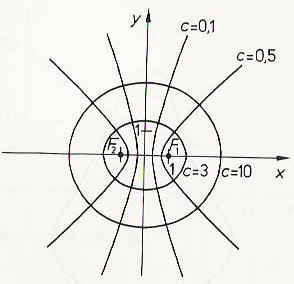
\includegraphics[height=4cm]{./bilder/orthoTrajekt.png}
}
& \parbox{14.5cm}{
Die orthogonalen Trajektorien schneiden alle Kurven der gegebenen Kurvenschar
$y=f(x,c)$ im rechten Winkel.\\
Die DGL $F(x,y,y')$ der Kurve bestimmen, anschliessend $y'$ durch
$-\frac{1}{y'}$ ersetzen.\\
$\Rightarrow$ ergibt die DGL der orthogonalen Trajektorien.\\
 \\
Die Kreise sind Orthogonaltrajektorien der Hyperbeln und umgekehrt.
}
\end{tabular}
